\documentclass[a4paper]{article}

\usepackage{amsmath, amsfonts, amssymb}
\usepackage{graphicx}

\usepackage{xepersian}
\settextfont{B Lotus}

\begin{document}
\begin{center}
	\large
	 به نام خدا\\
 یادگیری ماشین\\
 تمرین چهارم
 
 \normalsize
 ایمان رسولی پرتو\\
 \underline{810199425}
\end{center}
\begin{itemize}
	\item [1.] ‌
	\begin{itemize}
		\item[الف)]
		هدف توابع فعال‌ساز در شبکه‌های 
		\lr{MLP}
		غیرخطی کردن شبکه، افزودن قابلیت 
		\lr{backpropagation}
		و در نتیجه ایجاد قابلیت چند‌لایه‌سازی شبکه است. با چندلایه شدن و عمیق شدن شبکه امکان یادگیری توابع پیچیده‌تر با پارامترهای بیشتر فراهم می‌شود.
		
		اگر از توابع فعال‌ساز استفاده نشود، خروجی شبکه خطی خواهد بود و هر چقدر لایه‌ها افزایش پیدا کنند قابل ادغام با لایه‌های قبلی هستند و در نهایت خروجی همچنان ترکیب خطی از ورودی‌هاست. همچنین توانایی یادگیری توابع پیچیده را دیگر ندارد و عملیات 
		\lr{backpropagation}
		نیز دچار مشکل می‌شود.
	\item[ب)]
	اگر ورودی تابع
	\lr{sigmoid}
	بسیار بزرگ یا کوچک باشد، تغییرات خروجی کم است به این مغنی که گرادیان نزدیک به صفر می‌شود. این داستان باعث کندشدن سرعت همگرایی می‌شود.
	
	محدود بودن خروجی تابع 
	\lr{sigmoid}
بین 0 و 1 و مرکزیت صفر نداشتن باعث آپدیت‌های غیربهینه در 
	\lr{gradient descent}
	می‌شود که باعث کندشدن سرعت همگرایی می‌شود.
	
	یکی از جایگزین‌ها تابع فعا‌ل‌ساز
	\lr{ReLU}
	می‌باشد.‍ این تابع مشکل ورودی کوچک و بزرگ را برطرف می‌کند.همچنین پیاده‌سازی ساده‌تری نسبت به 
	\lr{sigmoid}
	دارد و بهینه‌تر است.
	
	جایگزین مناسب دیگر
	$\tanh$
	است که مرکزیت صفر دارد و آپدیت‌های گرادیان را بهینه‌تر انجام می‌دهد.
	\item[ج)]
	چون دو ویژگی داریم شبکه دو ورودی خواهد داشت. چون سه کلاس داریم شبکه سه کلاس دارد. داده‌ها با دو خط از هم جدا می‌شوند و یک لایه میانی کافی است. در لایه خروجی تابع فعال‌ساز
	\lr{softmax}
	قرار می‌دهیم. در نتیجه شبکه به شکل زیر توصیف می‌شود:
	\begin{figure}[!h]
	\begin{center}
		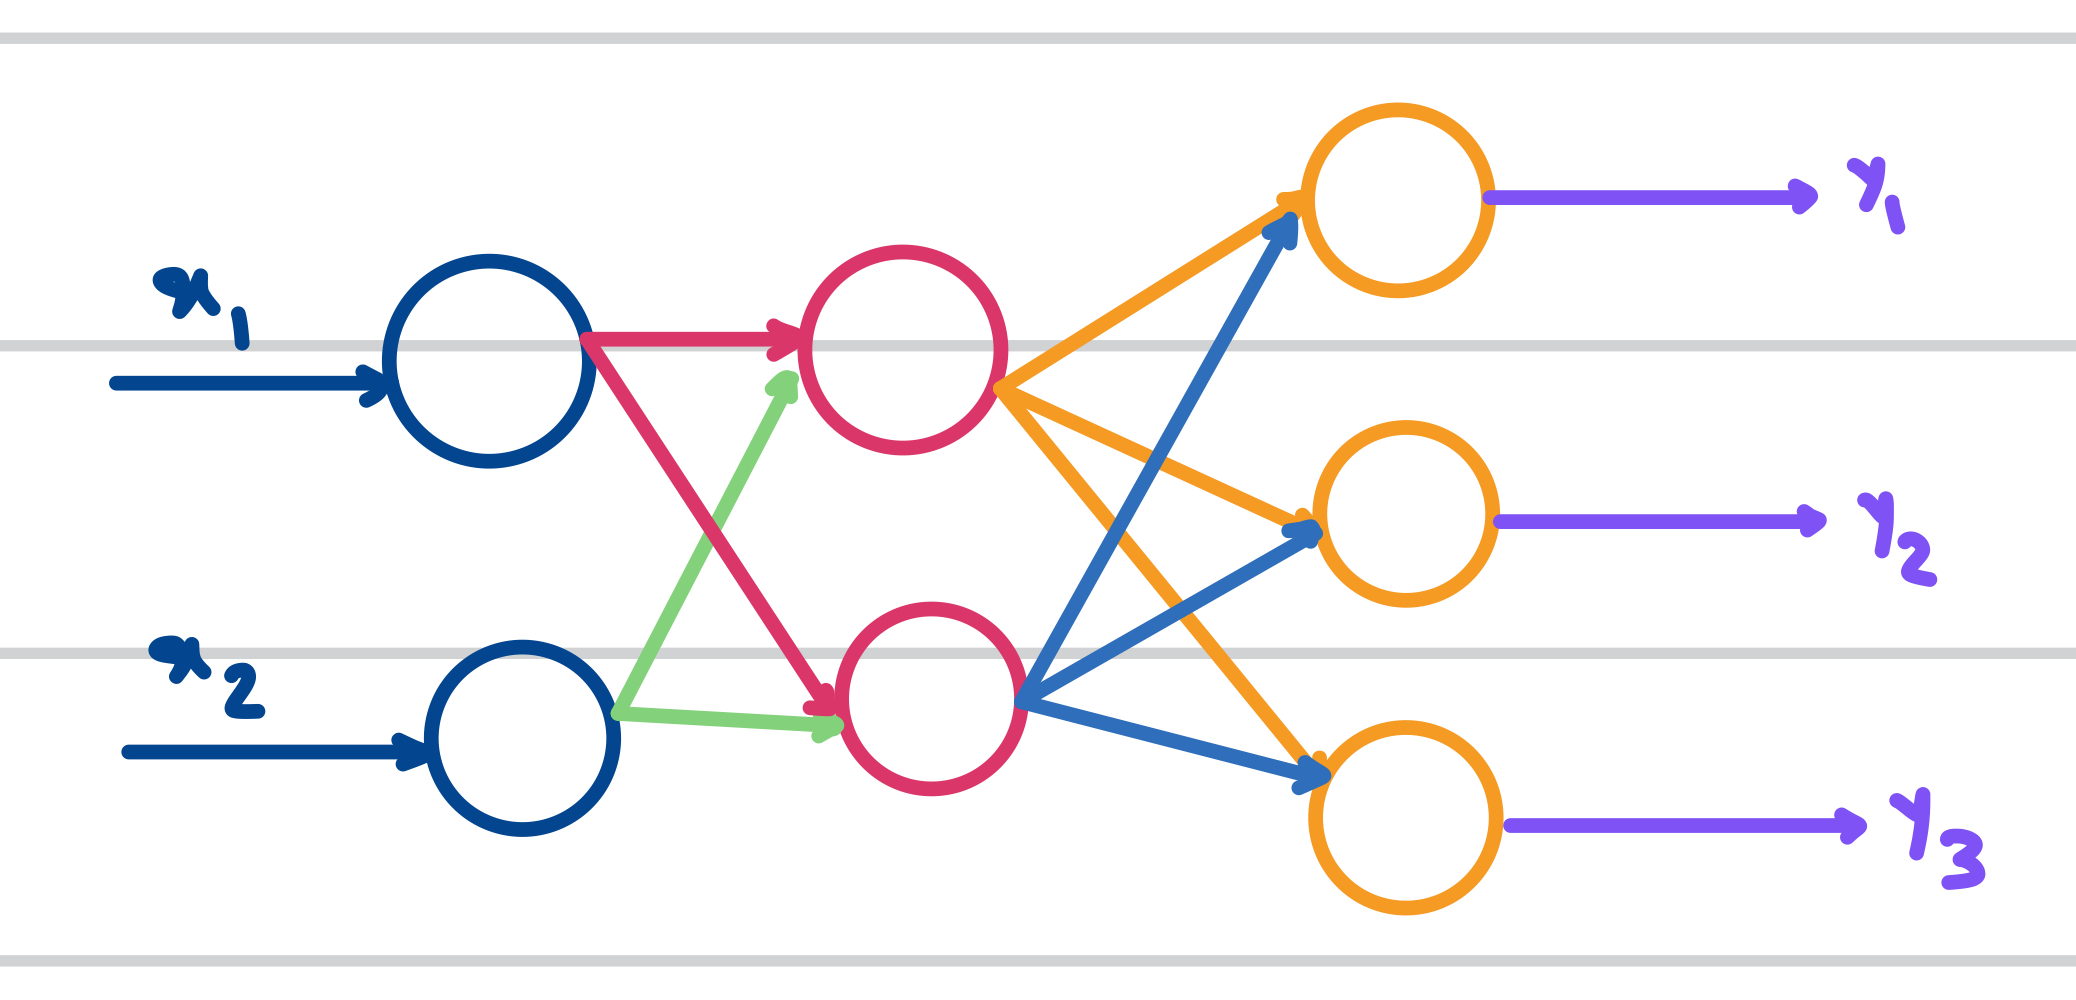
\includegraphics[height=4cm]{pic1.jpg}
	\end{center}
	\caption{ساختار شبکه طراحی شده}
	\end{figure}
	\newpage
	\item[د)]
‌
		\begin{figure}[!h]
		\begin{center}
			\includegraphics[height=9cm]{pic2.jpg}
		\end{center}
	\end{figure}
	\item[ه)]
	با استفاده از دو لایه می‌توان تابع پالس ایجاد کرد. هر تابع دلخواهی را می‌توان به شکل ترکیب خطی چند پالس بیان کرد. در نتیجه این مدل 
	\lr{MLP}
	می‌تواند یک 
	\lr{Universal appropriator}
	برای هر تابعی باشد.
		\begin{figure}[!h]
		\begin{center}
			\includegraphics[height=5cm]{pic3.jpg}
		\end{center}
	\end{figure}
	\end{itemize}
	\newpage
	\item[2.] ‌
	\begin{itemize}
		\item [الف)]‌
		\begin{figure}[!h]
		\begin{center}
			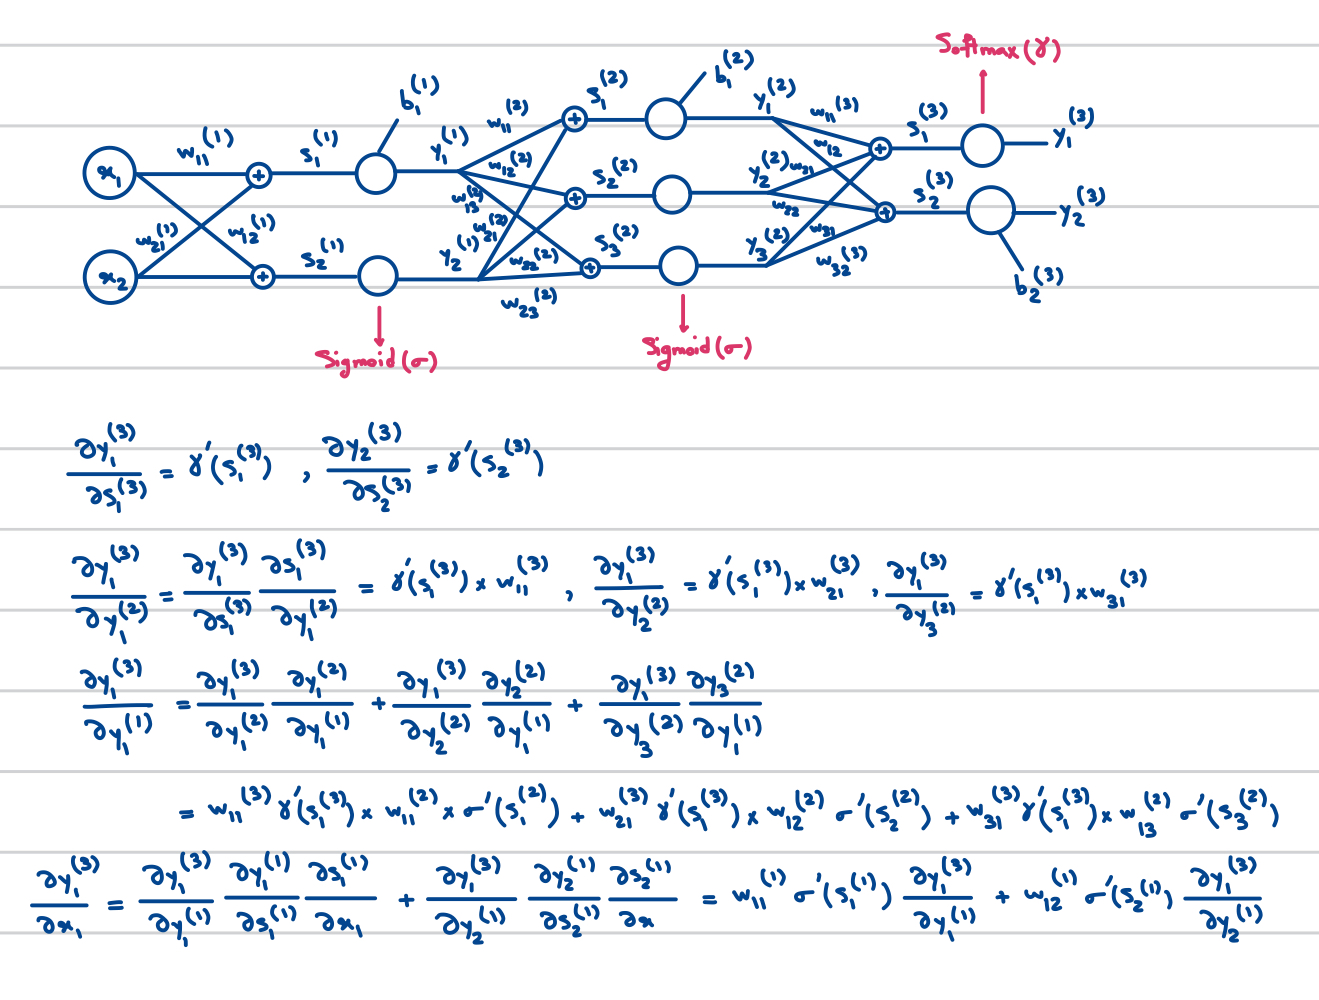
\includegraphics[height=9cm]{Pic4.jpg}
		\end{center}
		\end{figure}
		\item[ب)]‌‌
		
		\lr{\textbf{Stochastic gradient descent}}
		: مشابه الگوریتم 
		\lr{Gradient descent}
		می‌باشد. در هر تکرار بجای استفاده از کل داده‌ها برای محاسبه گرادیان تنها از یک نمونه یا یک زیرمجموعه از کل داده‌ها استفاده می‌شود. اینکار باعث کاهش حجم محاسبات و افزایش سرعت الگوریتم می‌شود.\\
نحوه کار: الگوریتم با مقداردهی اولیه به وزن‌ها آغاز می‌شود سپس یک داده یا زیرمجموعه‌ای از کل داده‌ها به شکل تصادفی انتخاب می‌شود. براساس داده(داده‌های) انتخاب شده، گرادیان محاسبه شده و وزن‌ها آپدیت می‌شود. این مراحل (غیر از مقداردهی اولیه) تا زمان همگرایی تکرار خواهد شد.

\lr{\textbf{Newton–Raphson method}}
: این الگوریتم یک روش تکراری برای محاسبات ریشه توابع حقیقی است.\\
نحوه کار: ابتدا یک نقطه به شکل تصادفی به عنوان نقطه شروع انتخاب می‌شود. سپس مشتق تابع در آن نقطه محاسبه می‌شود و نقطه طبق رابطه زیر به‌روزرسانی می‌شود:
\[
	x_{n+1} = x_n - \frac{f(x_n)}{f^{'}(x_n)}
\]

تا زمان همگرایی الگوریتم این روند تکرار خواهد شد.
	\end{itemize}
	\newpage
	\item[3.]‌
	\begin{itemize}
	\item[الف)]
ویژگی 
			\lr{Transitional in-variance}
در این شبکه‌ها به این معناست که اشیا فارغ از موقعیت و محل قرارگیری قابل تشخیص هستند.
	\item[ب)]
	در لایه‌های
	\lr{Convolution}
	فیتر روی تصویر حرکت کرده و میزان شباهت را با پنجره‌ای از تصویر که روی آن قرار گرفته می‌سنجد در نتیجه اگر جسم وسط یا گوشه تصویر قرار گرفته باشد باز هم توسط این شبکه‌ دیده خواهد شد.\\
	در لایه‌های
	\lr{Pooling}
	خروجی فشرده می‌شود. این امر وابستگی جسم به موقعیت تصویر را کاهش می‌دهد.
	\item[ج)]
	شبکه 
	\lr{MLP}
	را در چهار لایه با 
	\lr{activation function}
	های 
	\lr{ReLU}
	و
	\lr{sigmoid}
	در لایه آخر طراحی می‌کنیم. با 
	\lr{train}
	کردن شبکه به دقت $0.9796$ می‌رسیم.\\
	با طراحی شبکه
	\lr{LeNet}
	به دقت $0.9842$
	می‌رسیم.
	با شیفت دادن عکس‌ها و پیش‌بینی توسط دو مدل می‌بینیم که شبکه 
	\lr{LeNet}
	نسبت به تغییر موقعیت عدد در عکس مقاوم است و دچار خطا نمی‌شود.
	\begin{figure}[!h]
		\begin{center}
			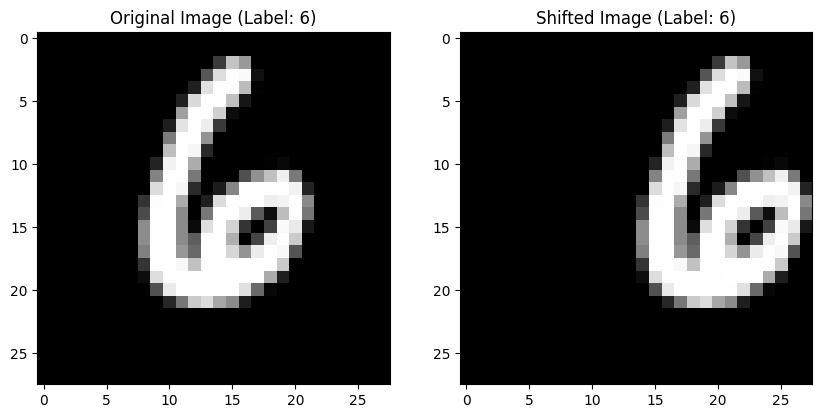
\includegraphics[width= 10cm]{Pic8.png}
		\end{center}
		\caption{تصویر شیفت داده شده در کنار تصویر اصلی}
	\end{figure}
	\begin{figure}[!h]
		\begin{center}
			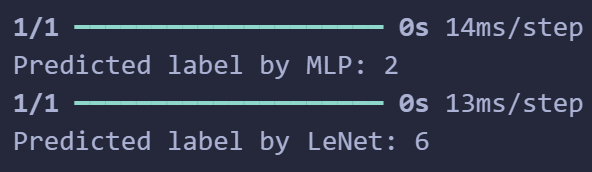
\includegraphics[width= 8cm]{Pic9.png}
		\end{center}
		\caption{نتایج پیش‌بینی توسط دو مدل}
	\end{figure}
	\newpage
	\begin{figure}[!h]
		\begin{center}
			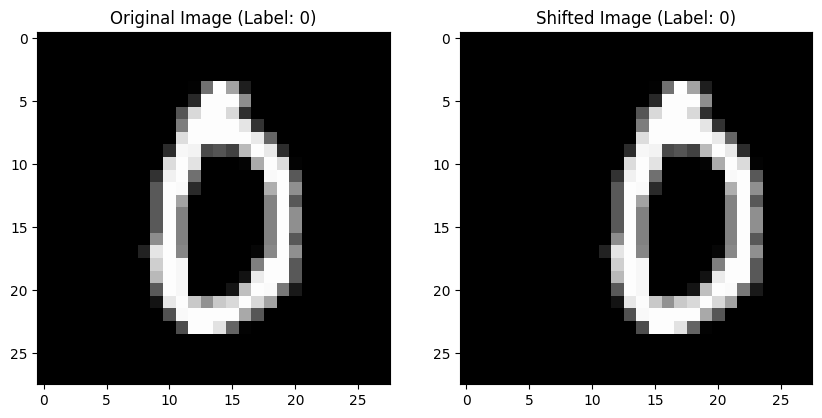
\includegraphics[width= 12cm]{Pic10.png}
		\end{center}
		\caption{تصویر شیفت داده شده در کنار تصویر اصلی}
	\end{figure}
	\begin{figure}[!h]
		\begin{center}
			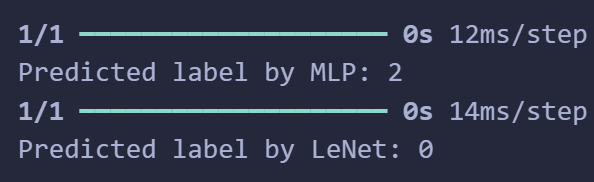
\includegraphics[width= 8cm]{Pic11.png}
		\end{center}
		\caption{نتایج پیش‌بینی توسط دو مدل}
	\end{figure}
		
با توجه به نتایج فوق مشاهده می‌کنیم که شبکه
	\lr{MLP}
	تصویر شیفت داده شده را اشتباه پیش‌بینی می‌کند اما شبکه
	\lr{LeNet}
	نسبت به شیفت مقاوم بوده و به درستی نتیجه را پیش‌بینی می‌کند.
	\end{itemize}
	\newpage
	\item[6.]‌
	\begin{itemize}
		\item[1-] تابع چاپ داده از دیتاست
		\begin{figure}[!h]
		\begin{center}
			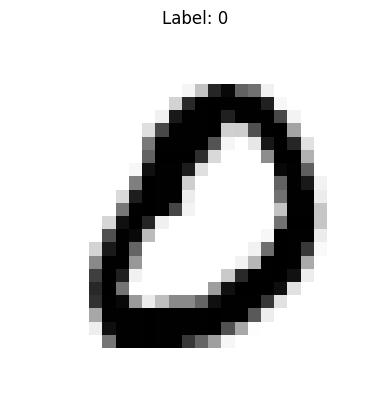
\includegraphics[height=6cm]{Pic5.png}
		\end{center}
		\end{figure}
		\item [2-]
		با توجه به نتایج 
		\lr{grid search}
		و 
		\lr{score}
		بهترین کرنل، کرنل
		\lr{RBF}
		خواهد بود.(نتایج و پارامترهای هر مدل در کد چاپ شده)
		\item [3-]
		با آموزش کرنل 
		\lr{RBF}
		روی داده‌های آموزشی خطای آموزشی $0$ و خطای تست $0.0869$ بدست می‌آید.
		\item [4-]
		خطای ناشی از اعمال 
		\lr{Logistic regression}
		روی داده‌های تست $0.1477$
		بدست می‌آید. این خطا نشان دهنده این است که
		\lr{SVM}
		عملکرد بهتری دارد.
		\item[5-]
		‌
				\begin{figure}[!h]
			\begin{center}
				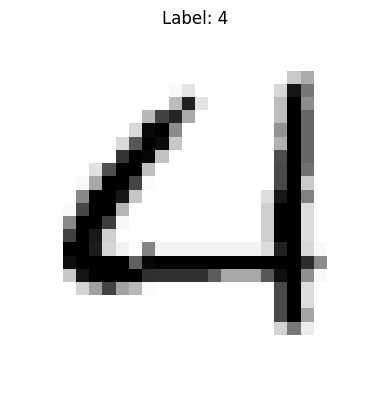
\includegraphics[height=6cm]{Pic7.png}
			\end{center}
			\caption{
				داده‌ای که توسط 
				\lr{SVM}
				به درستی و توسط 
				\lr{Logistic regression}
				به اشتباه طبقه‌بندی شده است
			 }
		\end{figure}
	\end{itemize}
\end{itemize}
\end{document}